\documentclass[oneside,11pt]{amsart}
\usepackage[utf8]{inputenc}%
\usepackage[english]{babel}%
\usepackage{amsmath,amssymb,amsthm,amsfonts}%
\usepackage[unicode]{hyperref}%
\usepackage{mathrsfs,bbm}%
\usepackage{paralist}
\usepackage{color}
\usepackage{longtable}
\usepackage{array}
\newcolumntype{L}[1]{>{\small\raggedright\arraybackslash}m{#1}}
\newcolumntype{T}[1]{>{\footnotesize\raggedright\arraybackslash}m{#1}}
\usepackage{stmaryrd}%
%\usepackage{refcheck}
\usepackage{graphicx}
\usepackage[DIV17]{typearea}
\usepackage{multicol,tikz}
\usepackage{datetime}
\usepackage{cleveref}

\usepackage[shadow]{todonotes}

\usepackage{etoolbox}
\patchcmd{\section}{\scshape}{\Large\itshape\bfseries}{}{}

\usepackage{caption}
\captionsetup{labelformat=empty,labelsep=none}

\hypersetup{
  colorlinks=true,
  linkcolor=blue!50!red,
  urlcolor=green!60!black
}

%%%%%%%%%%%%%%%%%%%%%%%%%%%%%%%%%%%%%%%%%%%%%%%%%%%%%%%%%%%%%%%%%%%%%%%%%%%%%%%%%%%%%%%%
\synctex=1
%%%%%%%%%%%%%%%%%%%%%%%%%%%%%%%%%%%%%%%%%%%%%%%%%%%%%%%%%%%%%%%%%%%%%%%%%%%%%%%%%%%%%%%%
%%%%%%%%%%%%%%%%%%%%%%%%%%%%%%%%%%%%%%%%%%%%%%%%%%%%%%%%%%%%%%%%%%%%%%%%%%%%%%%%%%%%%%%%
\newcommand{\score}[1]{\textit{#1}\addtocounter{totalscore}{#1}}
\newcommand{\razdel}[1]{\smallskip\underline{\textbf{#1:}}\smallskip}

\newcommand{\note}[1]{{\sf{}\color{blue}(#1)}}

\begin{document}

\title[MATH 7310: REAL ANALYSIS AND LINEAR SPACES I]{MATH 7310: REAL ANALYSIS AND LINEAR SPACES I}
\author{Leonid Petrov\\Spring 2019}
\date{Compiled on \today, \currenttime.\\An up to date syllabus is always on \texttt{GitHub} at \url{https://github.com/lenis2000/Syllabi/blob/master/Syllabus_7310_s19.pdf}. For direct PDF download use \href{https://github.com/lenis2000/Syllabi/raw/master/Syllabus_7310_s19.pdf}{\texttt{this link}}.
	\LaTeX{} source with \textit{changes} to the syllabus is \href{https://github.com/lenis2000/Syllabi/blob/master/Syllabus_7310_s19.tex}{\texttt{here}}
(click ``History'').}
\maketitle

\bigskip

\section{Graduate real analysis}
\bigskip

This course introduces students to basic analytic tools used across all of mathematics:
\begin{itemize}
	\item Measures, including the Lebesgue measure on the line
	\item Lebesgue integration
	\item $L^p$ and Hilbert spaces
	\item Absolute continuity, differentiation of measures
\end{itemize}

Additional topics included in the course will range from applications to 
probability (e.g., theory of conditional expectations, Gaussian measures and Gaussian Free Field, \ldots)
to selected topics from classical analysis (orthogonal polynomials, numerical methods, steepest descent, \ldots),
as time permits.
Students' suggestions of additional topics are also welcome.

\begin{figure}[h]
	\includegraphics[height=.32\textwidth]{img/chebyshev.png}
	\caption{The first six Chebyshev polynomials of the first kind.}
\end{figure}

\subsection*{Prerequisites}

Single variable and multi-variable Calculus (limits and continuity,
differentiation and integration, series, uniform convergence, etc.), Linear
Algebra (vector spaces, linear mappings, matrices, determinants, etc.), and
some knowledge of set theory and topology of metric spaces. 


\section{Necessary information}
\bigskip

	\textbf{Class times:}   TuTh 2:00PM - 3:15PM in
	\emph{Kerchof Hall 317}

\medskip


\textbf{Exams:} Please do not make travel plans which conflict 
with the first midterm or the final exam.
\begin{itemize}
	\item \textbf{Midterm 1:} In-class on February 19 (class time).
	\item \textbf{Midterm 2:} Take home, due April 4.
	\item \textbf{Final exam:} Monday, May 6, 9-12.
\end{itemize}

\medskip

\textbf{Instructor:} Leonid Petrov
\medskip

\textbf{Email:} \email{petrov@virginia.edu} or \email{lenia.petrov@gmail.com}
\medskip

\textbf{Office:} 209 Kerchof Hall
\medskip

\textbf{Office hours:} 
Tuesday and Thursday 10-11am, except the weeks when I'm \href{https://lpetrov.cc/2018/05/travel-2019/}{\texttt{traveling}}.\footnote{Note:
this PDF has green clickable links.}
Also feel free to drop in with quick questions any time, or make 
appointments 
(you can make as many appointments as you want).

\medskip

\textbf{Course webpage:} 
This term we will be using Piazza for class discussion. The system is highly catered to getting you help fast and efficiently from classmates and myself. Rather than emailing questions, I encourage you to post your questions on Piazza. If you have any problems or feedback for the developers, email \email{team@piazza.com}.

Find our class page at \url{https://piazza.com/virginia/spring2019/math7310/home}

A collab page for homework submissions will also be set up.

\section{Books}

The exposition of each topic will follow one
of the following books:
\begin{itemize}
	\item \emph{Real analysis: modern techniques and applications}, by G.B. Folland
	\item \emph{Real and complex analysis}, by W. Rudin
	\item \emph{Real analysis: Measure Theory, Integration, and Hilbert Spaces},
		by E. Stein and R. Shakarchi
	\item \emph{Measure Theory and Fine Properties of Functions},
		by L. Evans and R. Gariepy
	\item \emph{An epsilon of room: pages from year three of a mathematical blog},
		by T. Tao
\end{itemize}
The first two books are considered ``main'', 
the other ones are optional but may be of use.
Lecture notes (in a hand-written format)
will be provided on Piazza. 


\end{document}

\section{A mathematical study of randomness}

How random is everything around us, and what chance do we have of understanding it? What to do when you're not certain, and how to do it right? How many falling stars will you see as you walk outside one beautiful night? 

Probability theory is a mathematical study of uncertainty. It is a rigorous foundation of statistics --- and many areas of human knowledge operate in a language of statistics nowadays (yes, and robots use it, too!). The course introduces fundamental concepts, ideas, and techniques of probability theory. It will provide you with the foundational mathematical knowledge needed to address the questions above and will help you develop intuition about randomness.


\begin{figure}[h]
	\begin{tabular}{ccc}
		\includegraphics[height=.32\textwidth]{img/Bond_percolation_p_51.png}
		&\hspace{10pt}\includegraphics[height=.32\textwidth]{img/Amas_de_percolation_gray.png}
		&\includegraphics[angle=90,height=.32\textwidth]{img/RW1.png}
	\end{tabular}
	\def\figurename{}
	\caption{Examples of random structures: bond percolation
	\href{https://en.wikipedia.org/wiki/Percolation_theory}{\texttt{close-up}}
	(left),
	at a \href{https://commons.wikimedia.org/wiki/File:Amas_de_percolation.png}{\texttt{larger scale}} (center),
	and
	a 
	\href{https://en.wikipedia.org/wiki/Random_walk\#Lattice_random_walk}{\texttt{random walk}}
	(see also a
	\href{https://upload.wikimedia.org/wikipedia/commons/f/f3/Random_walk_2500_animated.svg}{\texttt{simulation}} 
	of a random walk).
	\tiny{Note:
	this PDF has green clickable links, like in the previous sentence.}
	}
\end{figure}

\subsection*{What you will get from this course}

\begin{enumerate}[\bf{}1.]
	\item Mastery of basic probability concepts:
	\begin{enumerate}[(a)]
		\item What is a probability space and how to translate commonly-sounding problems into this language;
		\item How to count (in an advanced way) to compute probabilities;
		\item What is a random variable, a probability distribution,
		and what are their main quantitative properties;
		\item 
		How commonly encountered probability 
		distributions (binomial, Poisson, exponential, Gaussian) look like and behave,
		what are 
		their properties, and in which situations they typically arise.
	\end{enumerate}

	\item How large random systems behave, and what the 
	bell-shaped curve
	\raisebox{-8pt}{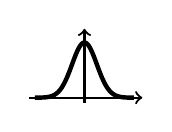
\begin{tikzpicture}
		[scale=.7]
		\draw[ultra thick, domain=-.9:.9] plot[samples=300] ({\x}, {2.7128^(-10*\x*\x)});
		\draw[->, thick] (-1.01,0)--(1.05,0);
		\draw[->, thick] (0,-.1)--(0,1.25);
	\end{tikzpicture}}
	has to do with this.
	\item How to describe and quantify the mutual dependence of random events,
	and how to use such a description 
	to infer properties of ``hidden'' random events.
	\item How to apply probability theory to model real-life processes like queues
	(consisting of people or requests at an internet server).
	\item How to collaborate on solving probability problems in pairs, small groups, and online,
	and present solutions clearly and efficiently.
	% \item How to design probability problems (for example, for the
	% final exam), and evaluate problems presented by others.
	\item In what ways probability theory is connected to science,
	engineering, and other branches of knowledge.
\end{enumerate}

\subsection*{Prerequisite} You should have taken at least one semester of calculus:
the study of random variables often requires single and double integrals
and infinite series.

\subsection*{What this course is and what it is not}

This course in probability \emph{theory} belongs to pure mathematics, with
rigorous definitions, calculations, and proofs. However, the objects which we
study are motivated by real-life applications, and so pure mathematical
arguments often appeal to our common sense understanding of these objects.
There will be opportunities to explore (and discover new) connections of the
theory studied in the course with the real world.

Also, this course does not thoroughly discuss \emph{applications to statistics}
Probability
theory focuses on developing the mathematical side, and statistics applies
these mathematical theories to real data (coming from observations). In this
course we will not discuss how to analyze data coming from observations ---
there are courses in statistics for that.

\section{Necessary information}

\subsection{Meeting times}{\ }\\

\begin{tabular}{|r|l|l|}
	\hline
	&Section 003&Section 001
	\\
	\hline
	\textbf{Class times}  & TuTh 12:30PM - 1:45PM &TuTh 2:00PM - 3:15PM
                       \\  & Monroe Hall 116 & Monroe Hall 116
                       \\ \hline
											 \textbf{Midterm 1}   & Thursday, \textbf{September 27}, 12:30-1:45 & Thursday, \textbf{September 27}, 2:00-3:15
                       \\  & Monroe Hall 116& Monroe Hall 116
                       \\ \hline
											 \textbf{Midterm 2}   & Thursday, \textbf{November 1}, 12:30-1:45 & Thursday, \textbf{November 1}, 2:00-3:15
                       \\  & Monroe Hall 116& Monroe Hall 116
                       \\ \hline
											 \textbf{Final exam}   &  Tuesday, \textbf{December 11} & Monday, \textbf{December 17}
											 \\ & 2:00PM-5:00PM &  9:00AM-12:00PM
                       \\  & Monroe Hall 116& Monroe Hall 116 
                       \\ \hline
\end{tabular}

\bigskip

	\textbf{Instructor:} Leonid Petrov

	\textbf{Email:} We use \texttt{Slack} instead, see \Cref{comm}

	\textbf{Office:} 209 Kerchof Hall

	\textbf{Office hours:} 
	Tuesday 11am-12pm, Thursday 10am-11am
	except the weeks when I'm \href{https://lpetrov.cc/2017/07/travel-2018/}{\texttt{traveling}};
	or by appointment (you can make as many appointments as you want;
	I am also available on \texttt{Slack} most of the time)

\subsection{About the instructor}
I am an assistant professor in the Department of Mathematics at UVA, and I've
been here since 2014. My research area is probability theory (very appropriate
for this course!). More precisely, I am using exact formulas to study large
random systems. I also like computer simulations of random systems like 
\href{https://d3m0khvr0ybm92.cloudfront.net/img/blog/heart/UVA_colors_small.png}{\texttt{this one}}.
I'm happy to tell you more if you're
interested.

\subsection{Textbook}

``Probability'' by Jim Pitman.
See also \Cref{success} below for discussion 
of how we'll use the textbook,
and for other helpful resources.

\section{Assessing your learning}

Learning mathematics means \emph{doing} mathematics: during class meetings, on your own, and in groups.
In this course, doing mathematics mainly amounts to solving problems.
There are four aspects which are assessed in this course:

\subsection{Homework (15\%)}

\begin{enumerate}[$\bullet$]
	\item Weekly homework will consist of textbook and other problems aligned with lectures, to
		help you practice new concepts and techniques. The homeworks are usually due on
		Thursdays, and will be assigned at least a week before the due
		date. 
	\item You are encouraged to work together on homework assignments. 
		This can be also done 
		online via \texttt{Slack}, which allows private groups of up to 9 people.
		Group work allows to 
		take advantage of challenge-defend discussions which help understand things
		better.  
		However, each student needs to submit her/his own homework
		assignments, and should work individually when writing them up to demonstrate
		the understanding of the material.
	\item The homeworks are graded ``coarsely'', that is,
		each homework will be assigned one of four grades: 
		\begin{equation*}
			\begin{tabular}{l|l|l|l|l}
				Grade & VG (very good) & G (good) & OK   & N \\
				\hline
				& \parbox{.21\textwidth}{All problems solved correctly with minor issues like arithmetic mistakes, and solutions explained
				in full detail}
				& \parbox{.21\textwidth}{Most problems solved correctly, and solutions explained in reasonable (close to full) detail}
				& \parbox{.21\textwidth}{ {\ }\\More than $3/4$ of problems attempted, many 
				solutions are incorrect, incomplete, or not explained in detail, 
				but the work displays adequate understanding of most of the material\\{}}
				& \parbox{.21\textwidth}{Work not submitted on time, or less than $3/4$ of problems 
				attempted, or most solutions are incomplete, or work clearly displays lack of understanding of most of the material}\\
				\hline
				\%    & 100\%          & 90\%     & 75\% & 0\%
			\end{tabular}
		\end{equation*}
		It is expected that most students 
		who put reasonable effort into the homework
		will get VG or G grades. 
	\item 
		The homework \emph{must be submitted only on Collab} (i.e., hard copies are not accepted). 
		Take pictures or scan your work,
		make sure it's readable,
		put it into a \emph{single PDF file with correct orientation},
		and upload it before the deadline.
%
		Submitting work like this has many benefits:
		(1) you retain a paper copy to
		prepare for tests; 
		(2) your submitted work is never misplaced or lost, and there is a digital trail;
		(3) the grading will be much faster and will allow me to immediately
		incorporate my impressions of homework solutions into in-class
		discussions. Moreover,
		(4) knowing how to scan and make a single PDF file is a
		valuable technical skill for the future: ask me and I can help you learn it.
\end{enumerate}

\subsection{Course engagement / quizzes (14\%)}

This includes short pop quizzes during lectures (at random days), 
and activity in \texttt{Slack} (including answering other student's questions).
There are no quizzes on the first week.
After that,
quiz days are determined by flipping independent random coins with 
probability of success $p=0.4$. 

One quiz with the lowest grade (or absence) will be dropped from the overall quiz grade.

\subsection{Midterm tests (2 tests each worth 18\%; 36\% in total)}

There are two midterm tests
held
during regular class times.
They have
similar taste as homework, and test basic knowledge of the material.

A two-sided letter size formula sheet, hand-written by yourself, is
allowed on each midterm test and on the final exam. Preparing this formula sheet
will help you review the material, and paint a systematic picture of the material in your mind.
Formula sheets cannot contain any photocopied or printed material
--- do everything by hand (of course, you can include any theorems, formulas, pictures, 
examples, etc).
The use of calculators (but not in mobile phones)
is allowed on the midterm tests and the final exam.

I encourage you to collaborate on test preparation, but needless to say that
during the test and the exam each student must work individually.

\subsection{Final exam (35\%)}

The final exam will be cumulative, but will put more focus 
on topics covered after the last midterm.

\subsection*{Letter grades}

The scale by which course percent grades are turned into course letter grades
will most likely be the following:
\begin{equation*}
	\begin{tabular}{l|l|l|l|l|l|l|l|l|l|l|l|l|}
		Grade      & $ A+	$ & $A	$ & $A-	$ & $B+	$ & $B	$ & $B-	$ & $C+	$ & $C	$ & $C-	$ & $D+	$ & $D	$ & $D-$ \\
		\hline
		Minimum \% & 100     & 93   & 89    & 86    & 82    & 79    & 76    & 72    & 69    & 66    & 62    & 59
	\end{tabular}
\end{equation*}
However, I reserve the right to slightly change this grade scale after the
final exam.
This may be needed
to better incorporate into the letter grade
possible fluctuations in the difficulty level of 
midterms and the final.

\section{Communication}
\label{comm}

\subsection{Email}

My email address is \href{mailto:petrov@virginia.edu}{petrov@virginia.edu}.

\subsection{Slack}
However, 
for the course
communication we will use \href{https://slack.com}{\texttt{Slack}} --- an
industrial standard of work messengers, with a web version and apps for all
platforms. This will make me more accessible if you have questions, and also
will let you answer questions of your fellow students. There will be course
content available \emph{only} on \texttt{Slack}, including scanned
lecture notes which I usually prepare for every class.

The course ``team'' is at \url{https://math3100-f18-uva.slack.com}. You'll get
an invitation to join by e-mail, and it is expected that you register.
Please
let me know if you have issues with access. 
It is also expected that you
will check announcements, and will participate in (or at least read)
the discussions of the course material.

Some things to note: 
\begin{enumerate}[$\bullet$] 
	\item \textbf{Population}:
		The \texttt{Slack} team will contain of students
		of all 3 sections of 3100 this semester which is at least 130 students.
		(However, all rules in this syllabus pertain to 2 of 3 sections 
		run by L. Petrov.)
	\item \textbf{Direct messages to me or Axel Saenz}:
		Direct messages are an excellent tool in \texttt{Slack} to communicate
		with me. If you're sending a first direct message, please 
		write your full name and which section you're from.
	\item \textbf{Direct messages to other students}:
		There are direct messages where you can talk to other students
		one-on-one. 
		You can also create private groups with up to 9 people, which
		is good for homework collaboration (but read \Cref{collaboration} on
		collaboration).
	\item \textbf{Privacy}:
		Although \texttt{Slack} is a messaging app, it should be used
		professionally, especially in public discussions. The app supports private
		direct and group messages. But please note that in principle the admin
		(i.e., myself) can obtain access to \textbf{all} direct messages between
		members of the team. 
		I assure you that this may be done only in extreme circumstances.
	\item \textbf{Email address}:
		You need an email address to use
		\texttt{Slack}, and it may be visible to other students. 
		Normally it's your UVA email address (I'll send an invite
		there). If you are not comfortable using your UVA email let me know
		and I'll be happy to send invite to another address.
		You can later change the email address yourself in the
		settings.
	\item \textbf{Notifications}:
		With \texttt{Slack}, it is easy to not miss important announcements and direct messages, 
		even if 
		you don't check it all the time --- 
		under the default settings, you will get notified (by email, too)
		about direct messages and mentions of your name. 
		All announcements will have mentions of everybody
		to draw attention. 
		Also, you can change notification settings, but please remember that
		there will be sometimes very important activity in \texttt{Slack} that you don't want to miss.
	\item \textbf{Public discussions}:
		Public messaging is separated into channels
		(\#general for class-wide questions/answers where you are welcome to post; 
		\#announcements and \#class-notes where I will post relevant information;
		special channels for homework discussion, midterm and final preparation, etc.).  
	\item \textbf{Many other features}: 
		\texttt{Slack} supports reminders out of the box. 
		You can ask it to remind yourself about a particular message, or 
		just set a general reminder. 
		With this, it is 
		easy to keep track of important messages
		(like class announcements or problems I'll post there).
		There are numerous third-party plugins one can add to \texttt{Slack}, and if you can 
		think of good ones to add, please let me know so I can add them.
\end{enumerate}

\subsection{Collab}

Solutions to homeworks / quizzes / midterms will be posted to both
\texttt{Slack} and Collab.  Grades will be posted to Collab as usual.  Homework
assignments will be posted to Collab and will be also announced in
\texttt{Slack}'s \#announcements channel. 
Your homework solutions can be submitted only through Collab, and will be graded there.

If you have anonymous comments on anything related to the course, you can make
them via Collab.

\section{How to succeed in the course}
\label{success}

\subsection{General things}

The best way to learn in the course is to 
come to all lectures, retain good memories 
of what was in there
(my brief class notes 
will be made available on \texttt{Slack}),
and do all the homework problems on your own or in collaboration.
This will prepare you well for pop quizzes, midterms, and the final exam.

\subsection{Main textbook}

The textbook \emph{``Probability'' by Jim Pitman} is an excellent resource 
to gain understanding of the course material. Some notes about it:

\begin{enumerate}[$\bullet$]
	\item You don't have to bring the textbook to all classes, 
		although this may be helpful sometimes. 
	\item I strongly encourage you to read the textbook. It includes many examples and
		extra exercises which augment the concepts discussed in class. 
	\item The textbook contains much more material than will be covered in classes, so it
		makes sense to come to all classes and see which parts of the textbook
		are covered and which are omitted.
\end{enumerate}

\subsection{Additional free textbook}

There is another (free) \emph{textbook} 
\emph{``Introduction to Probability'' by Grinstead and Snell}
with more problems and more material. It may be helpful if you want
a deeper understanding of some concepts, or if you want to read exposition of the familial material
in a different style (which might be very helpful for better learning!):
\begin{quote}
	Download: \url{https://math.dartmouth.edu/~prob/prob/prob.pdf}

	\noindent
	Accompanying web page: \url{https://www.dartmouth.edu/~chance/teaching_aids/books_articles/probability_book/book.html}
\end{quote}

\subsection{Extra reading}

The popular book
\emph{``How Not to Be Wrong: The Power of Mathematical Thinking'' by Jordan Ellenberg}
discusses how math touches every aspect of real life, and has 
numerous nice examples related to probability and statistics. 
I can recommend this nice book as a parallel reading. Some
examples I learned from this book might be mentioned in class.
(It absolutely not required that you buy or read this book.)

\subsection{Other resources}

There is a number of online resources which may help you while doing the homework:
Khan Academy, Wikipedia, and many other 
places contain lots of basic material on probability theory. Google
in general
is also a valuable resource.

\subsection{Office hours and \texttt{Slack}}

I am available during office hours to answer questions on the content of the 
course, clarify various points, and I can also help you with the homework assignments. 

Moreover, I am generally available in \texttt{Slack} for quick questions.
Note that if you post a question to the \#general channel, 
you also have a chance to get help from your fellow students!

\subsection{Tutoring center}

The Math Department Tutoring Center is available for helping students in this course: 
see \url{http://people.virginia.edu/~psb7p/MTCsch.html}
for more information and schedule. 

\subsection{Collaboration on homework assignments}
\label{collaboration}

Group work on homework problems is allowed and strongly encouraged.
Discussions are in general very
helpful and inspiring. Nevertheless, before talking to others, get well started
on the problems, and contribute your fair share to the process. 

When completing the written homework assignments, everyone must write up his or her own
solutions in their own words, and cite any reference 
(other than the textbook and
class notes) that you use. Quotations and citations are part of the Honor Code for both UVa
and the whole academic community. 

It is very important that you truly understand the homework solutions you hand
in, otherwise you may be unpleasantly surprised by your in-class test results.

\section{Approximate course schedule}

\noindent Add/drop information: \url{http://www.virginia.edu/registrar/reginst1188.html#Deadlines}
\smallskip

\noindent \textbf{NOTE: Please don't make travel plans conflicting with 
the midterms or the final exam}

\bigskip

\begin{quote}
	The course has 3 ``pillars'': central limit theorem for Gaussian approximation, 
	Poisson processes, and conditional expectations. 
	Plus there are several technical things to learn: random variables, expectations as integrals, 
	joint distributions, etc.
\end{quote}

\bigskip

\begin{enumerate}[\bf{}{[}week 1{]}]
	\item 8/28, 8/30.
		Introduction. 
		What is probability theory. 
		Sections 1.1--1.3

	\item 9/4, 9/6. 
		Advanced counting. 
		Conditional probability and independence. 
		Sections 1.1--1.4

	\item 9/11, 9/13.
		Advanced counting. 
		Bayes' rule. 
		Repeated trials. 
		Sections 1.5, 1.6, and 2.1.
		
	\item 9/18, 9/20.
		Binomial distribution. 
		Gaussian approximation. 
		Sections 2.1, 2.2

	\item 9/25.
		Random variables. 
		Expectation and conditional expectation. 
		Sections 3.1--3.3, and 6.1

		\textbf{9/27 --- midterm 1; covers sections 1.1--1.6, 2.1, 2.2}

	\item 10/2, 10/4.
		Random variables. 
		Expectation and conditional expectation. 
		Sections 3.1, 3.2, 3.3, and 6.1

	\item 10/11.
		Variance, Chebyshev inequality, central limit theorem (normal approximation).
		Continuous distributions.
		Sections 3.3, 4.1.
		
	\item 10/16, 10/18.
		Poisson distribution and Poisson process. 
		Coin tossing and geometric distribution. 
		Sections 2.4, 3.4, and 3.5

	\item 10/23, 10/25.
		Poisson distribution and Poisson process. 
		Coin tossing and geometric distribution. 
		Sections 2.4, 3.4, and 3.5

	\item 10/30, 11/1.
		Poisson processes, geometric, exponential and gamma distributions. 
		Sections 2.4, 3.3, 3.4, 3.5, 4.1, and 4.2.
		
		\textbf{11/1 --- midterm 2; covers sections 2.4, 3.1--3.5, 4.1, 4.2}

	\item 11/6, 11/8.
		Continuous distributions. 
		Change of variable and cumulative distribution function. 
		Sections 4.4 and 4.5
		
	\item 11/13, 11/15.
		Joint and conditional distributions. 
		Introduction. 
		Sections 5.1, 5.2.

	\item 11/20.
		Joint and conditional distributions. 
		Sections 6.1--6.4.
	
	\item 11/27, 11/29.
		Joint and conditional distributions. 
		Sections 6.1--6.4.
	
	\item 12/4, 12/6.
		Joint and conditional distributions. 
		Bivariate normal distribution. 
		Application to statistics. 
		Correlation. 
		Sections 5.3 and 6.5
\end{enumerate}

\section{Policies}

\subsection{Laptops and smartphones}

Please do not use laptops and smartphones during the class.
You won't need them to participate in the discussions, but they may easily distract 
you or other students (or me!). If you absolutely must use a laptop, please sit in the back row.

\subsection{\texttt{Slack} conduct}

Although \texttt{Slack} is a chatting app, it should be used professionally,
especially in public discussions.  The app also supports private direct
messages and I encourage to use them to collaborate on homework problems and
test preparation. But please note that in extreme circumstances the admin (i.e.,
myself) can obtain access to \textbf{all} direct messages between members of
the team.  So just don't say anything on \texttt{Slack} that you wouldn't say
in class.


\subsection{Late/make up work} Each assignment will have due date and time.
Late assignments are not accepted. There will also be no make up for the midterm test.
However, if you have special needs, emergency, or unavoidable conflicts, please
let me know as soon as possible, so we can arrange a workaround.

\subsection{Honor Code} The University of Virginia Honor Code applies to this
class and is taken seriously (in particular, 
see \Cref{collaboration} on homework collaboration).
Any honor code violations will be referred to the
Honor Committee.

\subsection{Special needs}

All students with special needs requiring accommodations should present the
appropriate paperwork from the Student Disability Access Center (SDAC). It is
the student's responsibility to present this paperwork in a timely fashion and
follow up with the instructor about the accommodations being offered.
Accommodations for test-taking (e.g., extended time) should be arranged at
least 5 business days before an exam.




\section{Policies}

\subsection{Laptops and smartphones}

Please do not use laptops and smartphones during the class.
You won't need them to participate in the discussions, but they may easily distract 
you or other students (or me!). If you absolutely must use a laptop, please sit in the back row.

\subsection{Late/make up work} Each assignment will have due date and time.
Late assignments are not accepted. There will also be no make ups for the midterm tests and the final exam.
However, if you have special needs, emergency, or unavoidable conflicts, please
let me know as soon as possible, so we can arrange a workaround.

\subsection{Honor Code} The University of Virginia Honor Code applies to this
class and is taken seriously (in particular, 
see \Cref{collaboration} on homework collaboration).
Any honor code violations will be referred to the
Honor Committee.

\subsection{Special needs}

All students with special needs requiring accommodations should present the
appropriate paperwork from the Student Disability Access Center (SDAC). It is
the student's responsibility to present this paperwork in a timely fashion and
follow up with the instructor about the accommodations being offered.
Accommodations for test-taking (e.g., extended time) should be arranged at
least 5 business days before an exam.




